\chapter{Artifact Development}
\label{ArtifactDevelopment}

With the theoretical design of the system complete,
the next step is to translate the design into a working prototype.
Therefore, this chapter will cover the development of the same,
including the iterative process and shining a light the difference between
the initial assumptions we made during the design phase and the reality of the implementation.

For this reason the chapter is divided into three sections.

First we need to discuss the constraints on the prototyping process,
this includes the existing infrastructure and the available hardware,
as this project as discussed in the \nameref{Introduction} is the extension and repurposing of an existing system,
build in a previous project.

Then the changes and improvements will be covered by the different steps of
the iterative prototyping, each step will be discussed in detail, the changes made and the reasoning behind them
as well as the issues encountered during the development process.

Lastly this chapter will conclude with a summary of the prototyping process,
the final state of the prototype and most importantly a reflection upon
the original design which has been deducted from the theoretical analysis
in contrast to the practical implementation,
which changes where made out of incorrect assumptions and which where made out of necessity.

% Previous work and existing infrastructure
\section{Previous Work}
\label{sec:previous_work}

As mentioned before, the goal of this project, besides to gather new knowledge
about the conjunction of \ac{HPC} and \ac{CC} is to extend the result of a previous project
by enabling it to become an Interactive Supercomputing Environment.

But as we will be take this previous system as a basis for our prototyping,
we will need to understand the design and architecture of the existing system,
and then decide which parts will be extended, which will be replaced, which will be removed
and which will be kept as they are.

The goal of the previous project was also a converged \ac{HPC} system based on the \textit{Arkouda} library,
but instead of focusing on an interactive environment,
it is based around a \gls{GitOps} workflow, where instead of the user interacting with the system directly,
the user submits code to a central version-control-system,
from where it gets cloned and packaged into container automatically.
If certain predefined conditions are met the workflow-system will then start
the container on the cluster and execute the code.

\pagebreak

\section{Existing Infrastructure}
\label{sec:existing_infrastructure}

\begin{figure}[!ht]
    \vspace{0.8cm}
    \centering
    \scalebox{0.35}{
        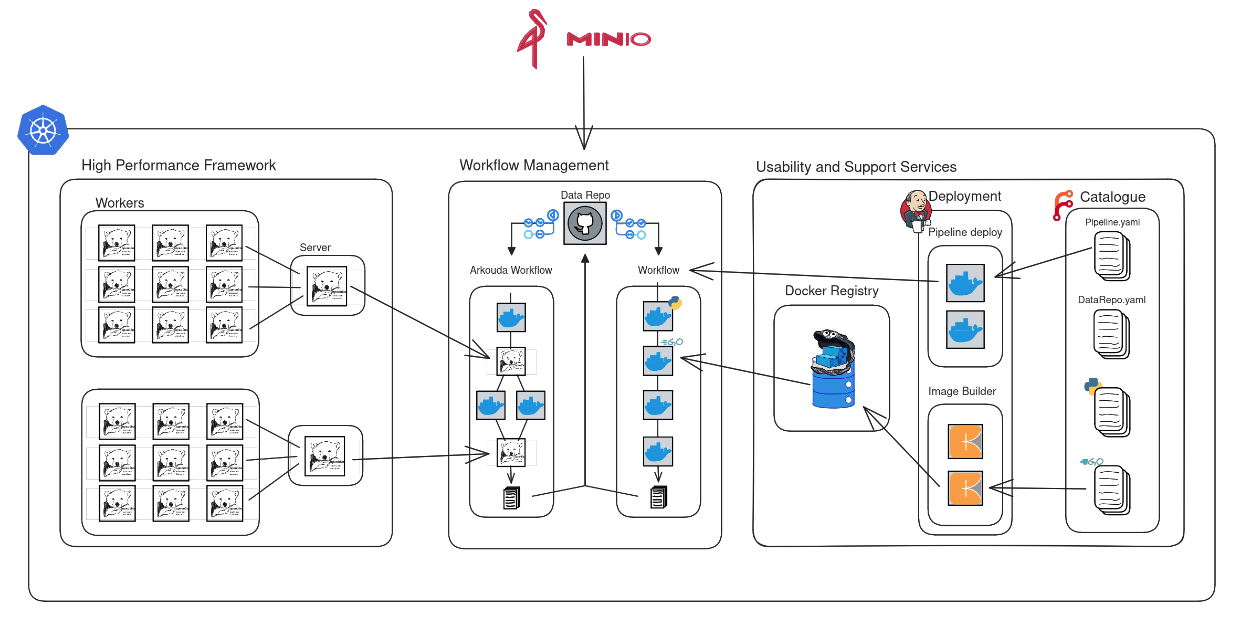
\includegraphics{./graphics/Pachykouda - High level architecture.png}
    }
    \caption{High level architecture of Pachykouda\protect\footnotemark}
    \label{fig:pachykouda_architecture}
\end{figure}
\footnotetext{Taken from \cite{eckerthDevelopmentDemonstrationProofofconcept2023}}

In the figure \ref{fig:pachykouda_architecture} we can see the high level architecture of the existing system,
it is split up in three relevant sections:

\begin{itemize}
    \item \textbf{Usability and Support Services:}  On the most tightern side we have the supporting infrastructure which also runs on the Kubernetes cluster,
          this includes the versioning system (Forgejo), the agent which builds the containers and workflows (Jenkins)
          and the storage for the containers images (Registry V2).
    \item \textbf{Workflow Management:} In the middle we have the workflow system(Pachyderm), which is responsible for the orchestration of the workflow,
          it starts the containers, manages their input and output and ensures the versioning of the results.
    \item \textbf{High Performance Framework:} On the left we have the Arkouda workers and the Arkouda server, which are the actual \ac{HPC} part of the prototype.
\end{itemize}

Beneath the service layer we have the Kubernetes cluster, which is responsible for the orchestration of the containers and managing the resources,
for both the computation as well as the all the other services, the only exception being the storage of the datasets versioned by
workflow system, which stores them in an external storage system, running on the a node of the same cluster, but not managed by Kubernetes.

On a hardware level we have a cluster of 20 nodes, connected by a 10Gbit/s network, in a star topology with a central switch.
Each node has a \textit{Intel Xeon E5-2680 v3 (48) @ 3.300GHz} and 270GB of RAM according to the information given in
the system stats. Also five of the nodes actually have an Infiniband capable network card, which could be used to test
the functionality of \ac{RDMA} capabilities of the Arkouda library, or jobs only requiring few cores but a lot of bandwidth.
On the Network abstraction layer the cluster is using the \textit{Flannel} network overlay, which provides a simple
layer 3 network between the nodes\footcite{flannelFlannelioFlannel2024}.


\section{Implication for the Prototype}
\label{sec:implications_for_prototype}
In the section \nameref{suggested_architecture} we created a suggestion for an architecture based on
our deductive reasoning we have done during the deductive analysis, as we now have discussed the environment
and existing infrastructure, we can now assess how our theoretical architecture can fit in a real world scenario.

The largest section of the previous system is the workflow management and its supporting infrastructure,
while this is also able to access the compute resources provided by the \ac{HPC} part of the system,
from a structural standpoint it will not impair the function of the system we are planning to building.
And the already running container \gls{registry} will also be useful for our prototype, as we will be able to use it to store the images of the containers we will be using.
Instead it demonstrates the high flexibility of kubernetes, being able to run many different services on the same cluster.


The \ac{HPC} part of the system we will be using as a basis for our prototype.
It is already able to run the Arkouda library, even though it is as of right now only accessible  through the workflow system.
while there is potential for optimization and improvement, it will provide a solid foundation for our work.

On the other hand, the cluster is mostly connected through a non \ac{RDMA} capable network,
which will limit the performance of the Arkouda library as discussed before.
While we do have two nodes with Infiniband network cards, we will only be able to use them for testing purposes,
but not in a full scale production like environment.
While there is little we can do about the available hardware,
Another consideration is the \ac{CNI} currently in use on the cluster,
as we might want to use a multi network setup, in oder to provide a separate network for the \ac{RDMA} capable nodes,
we would need to install \textit{Multus} or a similar \ac{CNI} on the cluster, which we then combine
with and \ac{RDMA} capable \ac{CNI} like \textit{OVN4NFV} or \textit{SR-IOV}.

While not a total necessity, it might be beneficial to have a container runtime available,
which is closer aligned with the \ac{HPC} part of the system, such as \textit{Singularity},
as it brings additional features such as native \ac{GPU} support and \ac{MPI} support, which might be useful for the prototype.

\pagebreak

% Iterative development process

\section{Iteration 1: Interactive Environment}
\label{sec:iteration_no1}

This is the first iteration of the prototyping phase.
The main goal is to get a \ac{MVP} running, what exactly this entails,
how it was achieved, how this relates to our \nameref{suggested_architecture}
and what the results of this iteration are, will be discussed in the following sections.


\subsection{Milestones and Goals}

The main goal of this iteration is to have an Arkouda environment running on the cluster,
which is accessible through a Jupyter client running on a local machine.

The milestones to be reached in order to achieve this goal are as follows:

\begin{enumerate}
    \item \textbf{Verification} While there is an existing installation running on the cluster,
          it has been running unattended for roughly a year and was originally intended for a different purpose.
          Therefore the first step is to verify that the installation is still operational and that the environment is still functional.
    \item \textbf{Deployment of Jupyter} The next step is to deploy a Jupyter server on the cluster,
          which is able to access the Arkouda environment. In order to do this a custom container
          image will need to be created, to run alongside the existing Arkouda environment.
    \item \textbf{Access from Local Machine} The final step is to make the service as low barrier as possible,
          by making it accessible from a local device.

\end{enumerate}

\subsection{Implementation}

\subsubsection{Verification}

Considering that the original installation was done as an experiment and has been running unattended for a year,
and has survived a hardware change and a resizing of the cluster, it is still operational.
One issue that was discovered during later steps was that during a final reformating of the repository,
the name variable of an \ac{RBAC} role was changed, which caused subsequent redeployment to fail,
but which was quickly resolved after the issue was identified\footcite{joneckerthFixingErroneousRBAC}.

\subsubsection{Deployment of Jupyter}

While there exist many ready made images for Jupyter,
the way the Arkouda client needs to be installed and configured requires a custom image to be created.
This is due to the fact that the Arkouda client library is not available through any standard package manager,
but needs to be installed from source\footcite{arkouda-repoArkoudaPydocSetup},
the same goes for the \textit{Chapel} compiler Arkouda is built on\footcite{chapel-lang.orgBuildingChapelChapel}.
Making the users do this manually would be a waste of time and compute resources.
Additionally in order to make the connection to the Arkouda environment,
\textit{IPython Kernel} needs to have access to current connection information at initiation and runtime.

\textbf{Image: }

The first step was to create this custom image,
the foundational image for this is the image provided by the \textit{Chapel} project\footcite{chapelChapelProfileDockera},
as it already contains a whole precompiled version of Chapel.
This is important as the Arkouda client library needs to use the binaries provided by Chapel,
in order to create the necessary shared objects for the Python bindings\footcite{arkouda-repoArkoudaPydocSetup}.
One thing which was not clear was, wether the Chapel binaries where still
needed after the shared objects were created, as our version only needs to act as a client.
After the chapel binaries and the Arkouda client library were installed,
the single user notebook server was installed and the \textit{IPython} kernel was
extended to load the required modules and establish the connection to the Arkouda environment as
well as to terminate the connection when the kernel is shut down.

\textbf{Deployment: }

In oder to get this custom image to work on the cluster,
a deployment script was created which has access to the internal network of the Arkouda Namespace and the
connection information needed to establish the connection to the Arkouda endpoint.
The container was then pushed to the clusters \gls{registry} and deployed to the cluster.

\textbf{Testing: }
\label{testing_iteration_no1}

To see wether the whole integration works the setup was
tested with scripts provided by the Arkouda project for demonstration purposes\footcite{arkouda-repoBearsRUsArkoudaNotebooksPlace}.
Unfortunately the system did not work as expected, the program terminating with the indication that the
requests of the client where not being answered by the server.
Due to no error messages being produced by the server,
the assumption being that the connection, going through all layers of the Kubernetes network stack,
was suddenly being dropped silently. After thorough investigation it was discovered that the
issue was instead caused by a bug in the Arkouda \textit{argsort} function causing a silent
crash of the process, when the function was called on a string array\footcite{hokiegeek2CommitsBearsRUsArkouda}.
For the initial prototype it was worked around by \gls{monkey patching} the function to use the \textit{NumPy} implementation
instead when the input is a string array.
This is not an ideal solution, as the \textit{NumPy} implementation is not distributed and therefore not as performant as the Arkouda implementation.
But this will get address in the next iteration, where the performance of the environment will be improved.
With this workaround in place the scripts provided by the Arkouda project where able to run successfully,
and the connection to the Arkouda environment was established and stable for the duration of the test.
More thorough testing in form of a benchmark for each of the operations will be done in the next iteration at \autoref{sec:iteration_no2}.


\subsubsection{Access from Local Machine}
The final step is to make the service accessible from a local device,
with the knowledge gained from the previous research, this was a simple task.
The Jupyter container was exposed to the outside world (the corporate intranet)
through a \textit{NodePort} service, which is now accessible from any device on the network.
In order to prevent unauthorized access, as the service is not secured by default,
additionally a password was set for the Jupyter server.

\begin{figure}[!ht]
    \centering
    \scalebox{0.32}{
        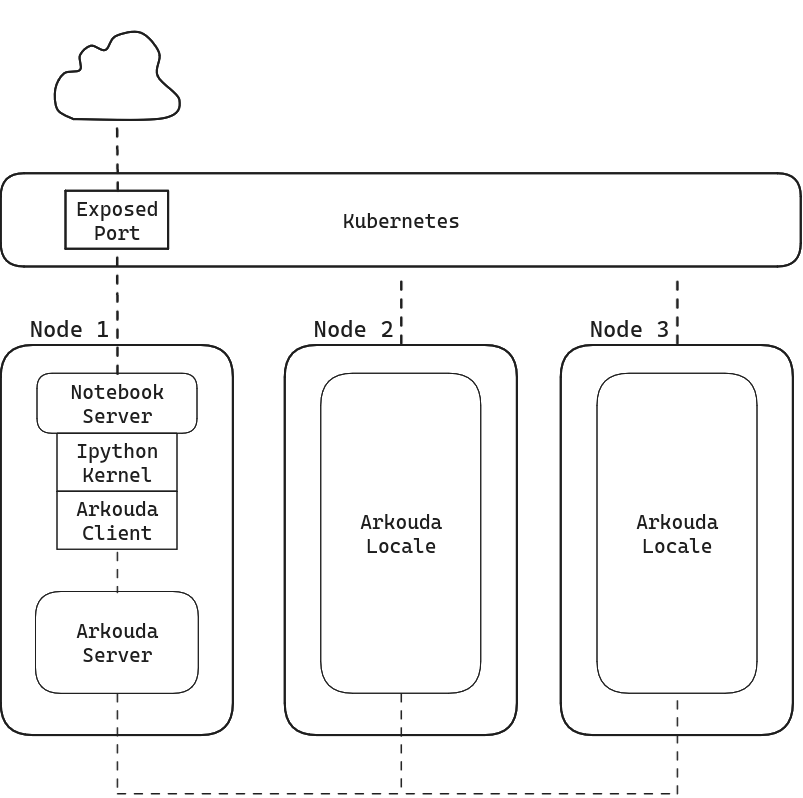
\includegraphics{./graphics/Jupyter-setup.png}
    }
    \vspace{0.6cm}
    \caption{ High Level Overview of the Jupyter Setup}
    \label{fig:juptyer_setup}
\end{figure}


In diagram \ref{fig:juptyer_setup} above is shown how the setup is structured, most importantly the Jupyter container is
the only container which is exposed to the outside world, the Arkouda container is only accessible from the Jupyter container.
Which itself connects to the \textit{Arkouda} Server only through a node internal network connection.
Each of the Ipython kernels has its own independent connection to the Arkouda server,
which is established at the start of the kernel and terminated at the end of the kernel.

Currently this system is completely ephemeral, as neither the Jupyter container nor the \textit{Arkouda}
\ac{GASNet} domain are being persisted.


\subsection{Evaluation of Results}


The Goal of this iteration was the creation of a \ac{MVP} of an interactive Arkouda environment
running on a multi node compute cluster, accessible through a Jupyter client.
While some issues where encountered during the implementation, the goal was successfully achieved.
The Arkouda environment is now accessible from any device on the corporate intranet,
and the connection to the Arkouda environment is stable and easily usable.

During the implementation some original assumptions made during the research a  nd the \Nameref{suggested_architecture}
but showed to be infeasible or incorrect and had to be adjusted.

% arkouda being young and promising might be a good idea to invest more time into it, especially since it still has some bugs which need to be fixed.

While using Chapel as the base for the high performance computing has shown to be a good choice,
the choice of using Arkouda to increase the ease of use for python developers has shown
that it is still quite young in comparison to long established libraries like \textit{NumPy},
and sometimes lacks \ac{QoL} features, like a simple pip based installation or a more verbose error handling.
But as it is unrivaled in the area of python based distributed computing on large scale data\footcite{ronaghanSqueezingPerformanceOut2020},
it is a promising library to invest more time into.

% original proposition was to use the arkouda container as a base layer, which was not possible due to ...
While there exits a container image to be used as an Arkouda client, which was intended
to be used as a base layer for the Jupyter container,
is build on the basis of an \ac{SMP} Chapel compilation.
If the Chapel binaries need to be replaced anyhow,
there is no reason not to use the right Chapel image from the start,
and building everything on top of that our self.

% Removing the reference to something that was not implemented
% % As of right now no autoscaling of the service
% As of right now there is only a single deployment of the services running on the cluster,
% with the express purpose of having more than one user at a time, utilizing 
% the cluster to its full potential, the service should be autoscaled.
% But in order to first have a comparable baseline, this was out of scope for this iteration,
% and as we are planning to use a topology aware deployment strategy, this should be addressed in \ref{sec:iteration_no3}.

% Fazit
\textbf{Conclusion:}

The goal of this iteration was to create a \ac{MVP} of an interactive Arkouda environment,
which is accessible from a local device. This goal was successfully achieved.
The environment is now accessible from any device on the corporate intranet,
and the connection to the Arkouda environment is stable and easily usable.

The initial assumptions made during the research phase and the \nameref{suggested_architecture},
where addressed and corrected during the implementation phase.
And during the implementation some new issues where discovered,
such as an issue with a function in the Arkouda library which will need to be addressed.
The next iteration will focus on improving the performance of the environment,
as during the testing the opportunity for improvement was discovered.

\pagebreak


\section{Iteration No 2: Performance Improvements}
\label{sec:iteration_no2}

In the previous section the prototype was successfully deployed and tested.
The next step is to move this from a \ac{MVP} to a more stable and performant environment,
this includes improving deployment and execution times,
as well as properly addressing previous workarounds.

\subsection{Milestones and Goals}

\begin{enumerate}
    \item \textbf{Deploy time:} As the image contains the entire Chapel compiler, its source code as wellas
          the Arkouda client library and its dependencies, the image is quite large. This slows down the deployment
          process, as the image needs to be transferred to the cluster and then unpacked. The goal is to reduce the
          size of the image to speed up the deployment process.
    \item \textbf{Container Runtime:} The current container \ac{CRI} is \textit{Containerd} which, while being
          lightweight, is not the fastest \ac{CRI} available. The goal is to switch to a faster \ac{CRI} more suited to
          \ac{HPC} workloads, such as \textit{Singularity}.
    \item \textbf{Investigating Arkouda Crash:} During the previous iteration, the Arkouda environment crashed
          when running the \textit{argsort} function on a string array. This was fixed by \gls{monkey patching} in the
          \textit{NumPy} implementation. The goal is to investigate the cause of the crash and fix it properly, to
          gain back the performance lost by using the \textit{NumPy} implementation.
    \item \textbf{Performance Testing:} In order to even quantify the performance in the first place,
          a way to measure the performance needs to be established. This will be done by running a set of benchmarks
          before and after the changes are made.
\end{enumerate}

\subsection{Implementation}

\subsubsection{Deploy time}

The time it takes a service from being requested and being available is crucial for the flexibility of a
Kubernetes cluster, as this determines how fast the cluster can adjust to changing workloads, increasing
demand or failures.  The current size of the image as reported by \textit{podman} is 3 GB, which is quite large,
for a simple client service. This is due to the fact that the e ntire Chapel project as well as all build tools are included in the image.
Having such a large image slows down the deployment process, as the image needs to be transferred and unpacked to the node.
One solution to this is prefetching the image on the nodes, is called \textit{image pre-pulling}.
Taking the time it takes to pull the image at an earlier time and storing a local copy on the node,
this way the image is already available when the service is requested.
This is feasible for small clusters with a low diversity of images, but the overhead of keeping local copies of
images locally, scales quadratically with the number of images and nodes, as each image needs to be stored on each node.
Therefore, we want to investigate by how much we can reduce the size of the image, to speed up the deployment process.

For this reason a script was written to measure the time it takes to deploy an image.
More about how this testing works can be found in the Performance Testing section of this iteration.

\begin{figure}[!ht]
    \vspace{0.8cm}
    \centering
    \scalebox{0.7}{
        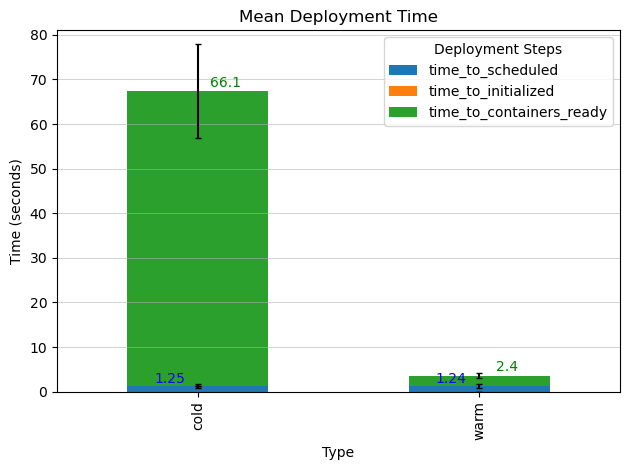
\includegraphics{./graphics/deployment-time-large-image.png}
    }
    \caption{Deployment time of a 2.86GB image\protect\footnotemark}
    \label{fig:deployment_time_large_image}
\end{figure}
\footnotetext{Data can be found in the project repo at \cite{joneckerthBachelorThesisProjecta}}

Figure \ref{fig:deployment_time_large_image} above shows the time the different steps of the deployment process take in seconds.
In blue is the time it takes from requesting the deployment of a service until Kubernetes assigns the pod to a node.
In the orange section we would see the time it takes the initialization containers of the pod to start.
The init-containers are needed to set up the namespace and network for the pod;
they pull and start the actual container image (see \Nameref{sec:containerization}).
However, as Kubernetes can only measure events with a resolution of seconds,
and these containers are ready in milliseconds, hey are too short to be measured reliably by Kubernetes.
Going from requested to ready in between the polling makes it seem like they are ready instantly.
The green section is the time it takes from the initialization containers being started to the whole pod
being able to accept requests. This includes the time it takes to pull the image from the registry, unpack it,
the start of the container and the time for the software inside the container to be ready to accept requests\footcite{kubernetes-docsPodLifecycle}.

With all else being equal we can clearly see the large difference between fetching the image from the registry,
and having the image already available on the node.
As container images are built out of \ac{COW} layers (see \Nameref{sec:docker}),
one can specifically target the layers which are the largest and try to reduce their size.
One thing to note is, that due to every command creating a new immutable layer,
one should try to chain commands together, to reduce the number of layers created.
So instead of creating a layer for the installation of a package, another layer for the usage
and a third layer for the removal of the package, one should chain these commands together in one layer to
result in a single layer containing only the artifact needed for the package.
The most effective method to reduce the size of an image besides, choosing smaller base images,
and being mindful of the layers created, is to use multi-stage builds.
This is a feature of the Dockerfile format that allows you to create multiple images from a single Dockerfile.
Its main use case is to build the project in one image and then copy the build artifacts to a second image.
This is useful as the first image can contain all the tools and dependencies needed to build the project,
while the second image can be a much leaner distribution, only copying the build artifacts from the first stage over,
reducing the overall size of the image significantly, while making the build process easier.

These practices were applied to our initial image, reducing the size from 2.86 GB down
to  710 MB, a reduction which is a largely due to the use of multi-stage builds,
replacing the Chapel image after the Chapel build was done. Additional size reduction
could be achieved by isolating the python modules after the Chapel build process and
moving them using a \ac{VENV} to the final image.

Overall the size reduction of the image had a significant impact on the deployment time as
can be seen in figure \ref{fig:deployment_time_small_image} below.,
reducing the median deployment time of a non-pre-pulled image from 63.47 to 19.7 seconds,
a reduction of 69\%, which is nice for a simple change in the Dockerfile.

\begin{figure}[!ht]
    \vspace{0.8cm}
    \centering
    \scalebox{0.7}{
        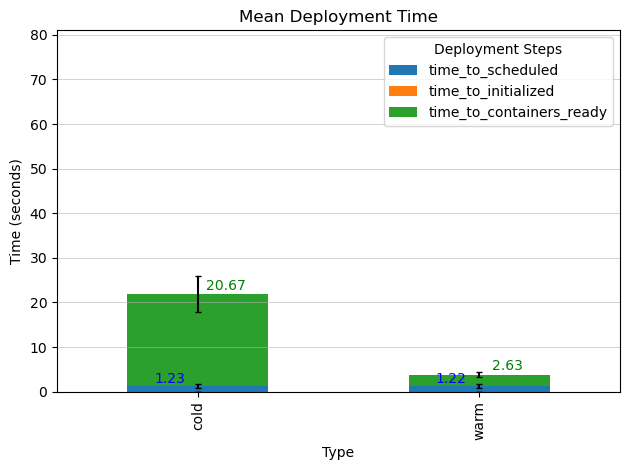
\includegraphics{./graphics/deployment-time-small-image.png}
    }
    \caption{Deployment time of a 710 MB image\protect\footnotemark}
    \label{fig:deployment_time_small_image}
\end{figure}

\footnotetext{Data can be found in the project repo at \cite{joneckerthBachelorThesisProject}}

But if we compare the difference the build makes on the prepulled image,
we can barely see any difference, both being around 2 seconds.
Being so close to a resolution of 1 second we can not see much of an effect.

As the images of the \ac{HPC} are taken from the Chapel and Arkouda projects,
they can also be given the same treatment, as the images are quite large as well.
While the Arkouda server and locale environment are even larger than the Jupyter image,
they are also much more complex, and rely on more than just the python bindings to work.
Multi-stage builds are especially important here since the tooling needed to compile
the chapel project alone already make up more than a gigabyte of the image.
It is also built on top of the original Chapel image, which is already quite large,
containing the precompiled Chapel binaries, saving the time of compiling Chapel during the build process.
But compiling both Chapel and Arkouda from source, using multi-stage builds,
and \ac{VENV}s to isolate the python modules, we were able to reduce the size of the image significantly.
The size of the Arkouda image was reduced from 3.88 GB to 1.08 GB, a reduction of 72\%
an effect which is even more important than the reduction of the Jupyter image,
as the Arkouda images will be running on each and every node in the cluster,
being scaled up and down as needed, making the flexibility of them quite important.


\subsubsection{Container Runtime}
\label{sec:container_runtime}

As can be seen from the diagrams above, the significant effect changing the size of the image has on the deployment time,
only effects the time it takes pulling and unpacking the image, but not the startup time or the time it takes for the software to be ready.
The setup time for a prepared container is mostly determined by the software inside the container as well as the overhead of container,
which is determined by the \ac{CRI} used.
WRewriting Jupyter notebook or a \ac{HPC} scale parallel processing framework like Chapel to be faster is certainly out of
scope for this thesis, however on the other hand changing the \ac{CRI} is a much more manageable task,
which will also might prove beneficial to later iterations as discussed in the \Nameref{suggested_architecture}.

Replacing the \ac{CRI} on a running Kubernetes cluster is akin to changing the engine of a car while it
is still running, as the \ac{CRI} is responsible for the runtime of the containers, and is responsible for
starting and stopping the containers, as well as managing the container's lifecycle.
Completely replacing an all-purpose \ac{CRI} like \textit{Containerd} with a
\ac{HPC} optimized \ac{CRI} like \textit{Singularity} might have unforeseen consequences.
Therefore, having both available on the same nodes, and utilizing whichever is more suited for the task at hand,
would be ideal.

Unfortunately, this step proved to be more difficult than anticipated,
as the \textit {Singularity} \ac{CRI} documentation claims to be able to run on a Kubernetes cluster,
which is not untrue;
But due to the singularity becoming a part of the open software foundation in 2015,
the project has been split into a community edition being maintained by volunteers,
and a completely rebranded version called \textit{Apptainer} which has moved away
from the \ac{HPC} space completely focusing now on subjects such as \textit{Sigstore} and Continuous Delivery.
The original version of \textit{Singularity} is still available on the \textit{Sylabs} website,
but has not been updated in the last 5 years, a fact which is not mentioned
when looking at the documentation\footcite{singularity-docsIntegratingKubernetesSingularity},
only visible when looking at the actual code of the project\footcite{singularity-repoSylabsSingularitycriSingularity}.
The version of \textit{Singularity} that is being maintained by the community, and more up to date,
is much smaller in scope and decided to focus their efforts to core projects,
abandoning the \ac{CRI} implementation\footcite{singularity-repoSylabsSingularitycriSingularity}.
While it technically still possible to run a cluster with \textit{Singularity} running as a \ac{CRI},
it is not possible  to do so for any version of Kubernetes beyond 1.26.
This is due to the fact that the \textit{Singularity} \ac{CRI} is based on the now deprecated version \textit{v1alpha2}
which was removed in version 1.26\footcite{kubernetes1.26releaseteamKubernetesV1262022}.


It is possible to run a \textit{Singularity} container without the \ac{CRI} on a Kubernetes cluster,
as it supports the \ac{OCI} standard, which means that one can convert a \textit{Singularity} image
to any other \ac{OCI} compliant image, and then run it on the generic \ac{CNI} of Kubernetes.
The features of \textit{Singularity} that made it originally so attractive for \ac{HPC} workloads,
such as its native support for \ac{GPU}s and \textit{Infiniband}
would need to be implemented the hard way, in Kubernetes itself, which then would defeat the purpose of using
a different \ac{CRI} in the first place.

\subsection{Investigating Arkouda Crash}

As we touched on in the previous iteration (\ref{testing_iteration_no1}) we had a problem with the Arkouda environment
crashing when a certain function is called on a string array. At that point in time, tracking down the error
proved time-consuming, and once enough information was gathered a workaround was found by \gls{monkey patching}
the function to use the \textit{NumPy} implementation instead(which can be found in the project repo\footcite{joneckerthBachelorThesisProjectb}),
while leaving the proper fix for the next iteration, as the primary goal was to get the system up and running.
After further investigation the hypothesis was that the error was not actually a bug in the code,
but a mismatch in the communication protocol between the Jupyter server and the Arkouda server.
While both were using the same version of the Arkouda library the Arkouda was originally
build when the system was set up during the "Pachykouda" project; the Jupyter server being build
during the first iteration of this project, there might have been some changes within the containers
since then.

As we have been relying on these containers provided by the Chapel and Arkouda projects,
we have little control over the versions and the variables used to compile the binaries.
Additionally, these images are quite large, slowing down the deployment as discussed in the first iteration.
To reduce the size of the images and to gain more control over the environment,
the images were rebuilt from scratch.
So a common base image was created, containing all the necessary files and binaries needed for the client, server and locale images.
From this base image, the corresponding images were created,
having an identical common environment but including only the necessary files
for the specific image to be created.
Thereby ensuring that the environment is the same for all images and have
the same version of the binaries and libraries at heart.

After the images were successfully brought to a state were they could be used as
a drop-in replacement for the original images, the client was tested again, and the error was gone.



\subsection{Performance Testing}
\label{sec:performance_testing}

Originally it was planned to test both the effect of the image size on the deployment time,
as well as the effect of the \ac{CRI} on the startup time and the execution time of the software.
Due to the fact that \textit{Singularity} only supports \ac{OCI} based execution on kubernetes,
there would be no relevant difference as both get converted into the same container format\footcite{opencontainerinitiativeImagespecSpecMd2024},
making the effort of converting the compute nodes to \textit{Singularity} inefficient in
the context of this project.

But testing the startup time was still possible and with the conversion of the Arkouda images and the
reduction of the size of the Jupyter image, having a good sense of how quickly the system is able to respond
to changes in the workload is still important.
The testing was done by utilizing Kubernetes "Pod Conditions" which are a set of states a pod
transitions through in its lifecycle, which can be used to monitor the state of the pod\footcite{kubernetes-docsPodLifecycle}.
Being able to query this information with the Kubernetes API, we can measure the time it takes for a pod to go from
start of the request to the pod being scheduled on a node, the time it takes for the pod to be initialized and the time it takes for the pod to be ready to accept requests.

So in order to compare hot and cold starts, it was needed to make sure that during the first run,
all of the images were not pre-pulled, and during the second run, all the images were pre-pulled,
the former needing to be wiped from the corresponding nodes each time.
The results of the testing can be seen in the diagrams above, and show a significant difference between the two,
with the pre-pulled images being ready in a fraction of the time of the non pre-pulled images.
The tests were done with a sample size of 400 with the images being deployed on the whole cluster,
and the results were then aggregated to show the median time it takes for the images to be ready.
The code\footcite{joneckerthBachelorThesisProjecte}, the notebook of the analysis\footcite{joneckerthBachelorThesisProjectd} and the raw data\footcite{joneckerthBachelorThesisProjectc} can be found in the project repo.


But as we are planning to compare the performance improvements of future iterations, it is important to
establish a baseline anyhow, for this reason a testing environment was set up and benchmarks were run on the cluster.
In order to do this, the Jupyter client was modified to run the micro benchmarks provided by the Arkouda project\footcite{arkouda-repoArkoudaRepoBenchmarks}.
The micro benchmarks test the performance of each of the major functions, such as \textit{argsort}, \textit{sum} and \textit{aggregate},
on all the supported data types. Getting a very fine-grained view of the performance of the Arkouda environment,
in each and every aspect.
As the cluster has four nodes which are theoretically \ac{IB} capable,
and will be enabled in the next iteration,
the benchmarks were limited to four nodes as well in order to have a fair comparison.
The tests were run with a problem size from $10^6$ to $10^{11}$ items per array,
in order to show how the performance behaves with increasing problem sizes.
% Additionally a comparison with the \textit{NumPy} implementation was done, 
% to show the advantages and disadvantages of a distributed array implementation, 
% in contrast to a classical single node implementation.

\begin{figure}[!ht]
    \vspace{0.8cm}
    \centering
    \scalebox{0.55}{
        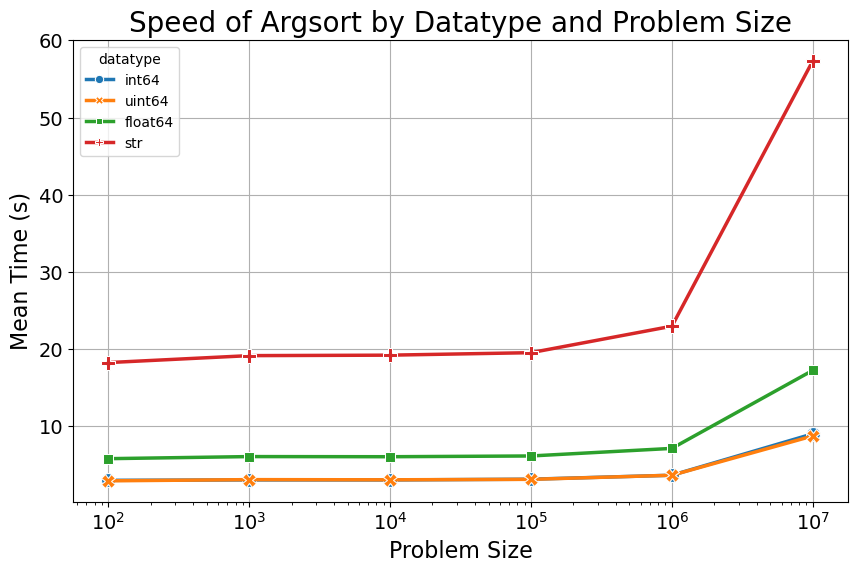
\includegraphics{./graphics/argsort.png}
    }
    \caption{Argosort by Problem Size}
    \label{fig:argsort}
\end{figure}
\footnotetext{Data available at: \cite{joneckerthBachelorThesisProjectf}}

The figure \ref{fig:argsort} above shows the how the performance of a tightly
coupled problem such as the \gls{argsort} function.
Here it can be seen how the time to solve the problem starts to increase exponentially,
corresponding to the problem size increasing by orders of magnitude for each test.

Another interesting aspect is the performance of the different data types,
as sorting a string array of the same length takes much longer than any other data type.
This is due to the variable length of strings in Arkouda, making the addressing
of the elements by index much more computationally expensive\footcite{arkouda-repoStringsArkoudaArkouda}

While \gls{argsort} implementing the sorting algorithm \textit{least-significant-digit radix sort}
demonstrates one of the worst cases for the performance an distributed system,
as it is a tightly coupled problem with a complexity of $O(w \cdot n)$,
were $w$ is the number of bits in the key and $n$ is the number of elements in the array.
The \textit{aggregate} function, shown in the diagram \ref{fig:agg_speed_by_datatype} below,
shows a much more diverse set of problems and how the performance of the system behaves with them.


\begin{figure}[!ht]
    \vspace{0.8cm}
    \centering
    \scalebox{0.55}{
        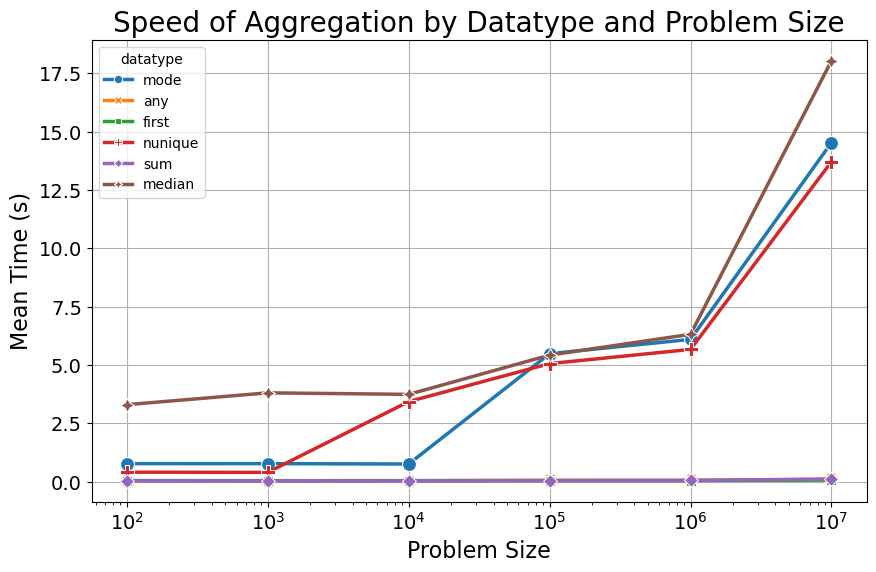
\includegraphics{./graphics/agg_speed_by_datatype.png}
    }
    \caption{Aggregated Speed by Data Type}
    \label{fig:agg_speed_by_datatype}
\end{figure}
\footnotetext{Data available at: \cite{joneckerthBachelorThesisProjectf}}

The figure \ref{fig:agg_speed_by_datatype} above shows clearly the wide gab in performance between
\textit{embarrassingly parallel} problems like \textit{sum}, \textit{any} or \text{first},
which are being split up into smaller problems and can be solved independently on each of the nodes,
without the need for any communication between them.
While less computationally expensive than \gls{argsort},
functions such as \textit{median} or \textit{mort} become time expensive,
as they can not be split up into smaller problems as easily.

So far the performance of the system has only been measured by the time it takes to solve
a problem of a certain length, but as the size of the elements themselves are not created equal,
or might even vary such as in the case of strings one should also take into account the actual
amount of data being processed.

Diagram \ref{fig:operation_data_transfer} is especially interesting as it shows the
clusters most extreme conditions. On one side the functions with the highest processing
rate and then the three functions with the slowest rate of processing.

\begin{figure}[!ht]
    \vspace{0.8cm}
    \centering
    \scalebox{0.6}{
        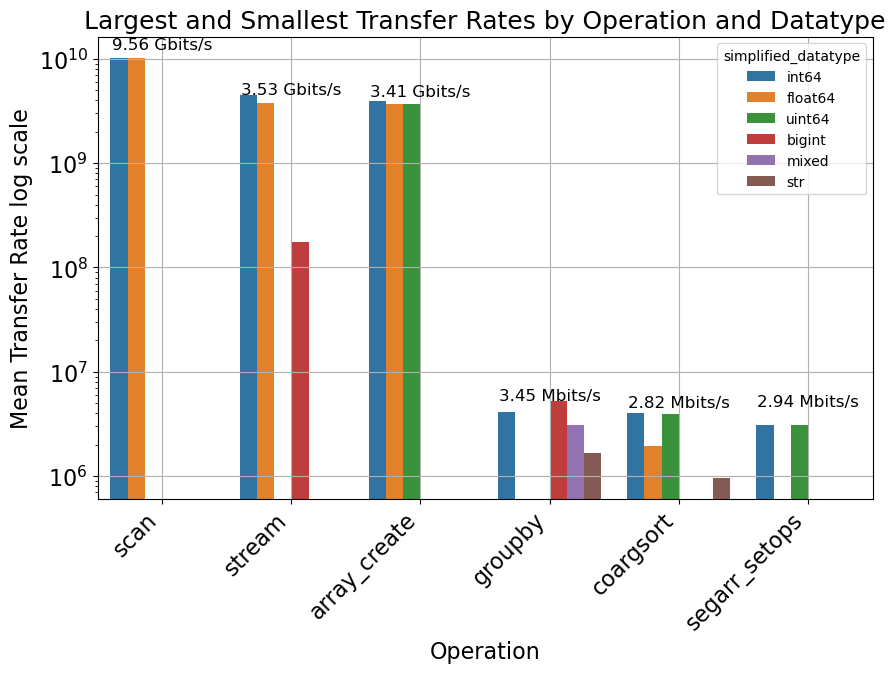
\includegraphics{./graphics/operation-data-transfer.png}
    }
    \caption{Operation Data Transfer}
    \label{fig:operation_data_transfer}
\end{figure}
\footnotetext{Data available at: \cite{joneckerthBachelorThesisProjectf}}

The speed of scanning the distributed array is essentially only limited by the speed of the underlying network,
as the data can be read in parallel from all nodes, and then aggregated on the client.
While the \textit{scan} function is very close the theoretical ideal of the network speed,
showing that the overhead of the whole network stack can be as low as 4.4\% under certain conditions;
The streaming function is not too far from the ideal processing speed of 30\%
of the network speed.
As the streaming function sends the \textit{axpy} operation to all nodes,
calculating $\displaystyle \boldsymbol {y} \leftarrow \alpha \boldsymbol {x}+ \boldsymbol {y}$.
Adding two arrays together while multiplying one of them by a scalar, this is a very simple and fast operation,
as each of the nodes can calculate the operation independently and then send the result back to the client.
The only delay being the time it takes to send the two arrays and receive the resulting array back.

The three arkouda functions which take the longest to process the data are
\textit{coargsort}, \textit{groupby} and \textit{segarr\_setopps}.
While \textit{groupby} directly calls the \textit{argsort} function and then performs
additional aggregations, \textit{coargsort} provides an index array just like \textit{argsort},
but instead of ordering it numerically it orders it by the order of another array.
As these functions just as \textit{argsort} are tightly coupled problems,
and rely on a lot of communication between the nodes, they are the slowest functions in the benchmark.
But the outlier in this case is the \textit{segarr\_setopps} function, which is a set operation on segmented arrays.
\textit{Segarr\_setopps} is even slower than complex sorting algorithm,
which seems counterintuitive at first, but the reason for this is that the function
has not been implemented for the distributed array yet \footcite{arkouda-docsSegArraysArkoudaArkouda},
and is being executed on the client negating the benefits of the distributed array implementation.

\subsection{Evaluation of Results}

The goal if this iteration was to move the \ac{MVP} to a more stable and performant environment,
reducing load times, fixing bugs and improving compute performance.
From this the need for a way to measure the performance in the first place was established.

The first goal, reducing the deploy-time by optimizing the image size of all parts of the system was
a complete success, with reductions in the size of the images around 70\% and the time to
deploy reduced significantly in the case of a non pre-pulled image.
While the original suggestion only intended to extend the images depending on our needs (see \Nameref{sec:container_image}),
during the prototyping phase the potential of large improvements were discovered,
and the decision was made to rebuild the images from scratch.

The second major goal, replacing the \ac{CRI} with \textit{Singularity} was not accomplished,
and the decision was made to not pursue this further,
as this would require updating a \ac{CRI} implementation which has been unsupported for the last 5 years.
While the performance increase would have had an impact on the container overhead,
a more significant impact would have been the native support for \textit{Infiniband} and \ac{GPU}s,
the former being especially important for \ac{HPC} workloads (see \ref{sec:networking_interconnects})
in but even more so with the current \ac{GASNet} implementation of Arkouda (see \ref{sec:gasnet}).
This gap in potential will be addressed again in the next iteration.

During the effort to rewrite the container images from scratch, the communication error was fixed,
and the Arkouda environment was running without any issues, passing all the unit tests and benchmarks.
The current theory being, that the issue was most likely due to a mismatch in the communication protocol,
between the jupyter server and the Arkouda server, which was fixed standardizing the versions across all images.

The last goal, establishing a baseline for the performance of the system was originally intended to be the basis
for the comparison between the \ac{CRI}s, but even though this was not possible, the benchmarks were still run,
in order to have a baseline for the performance of the system.

\subsection{Conclusion}

While some of the goals were successfully accomplished,
the goal of replacing the \ac{CRI} with \textit{Singularity} was not.
The performance of the image distribution was improved significantly,
and a baseline for the performance of the system was established.
The Arkouda environment was fixed and is now running without any issues.


\pagebreak

\section{Iteration No 3: Infrastructure and Interconnect}
\label{sec:iteration_no3}

\subsection{Milestones and Goals}

As has been discussed in the section \Nameref{sec:hpc_infrastructure} the second most important
aspect of a \ac{HPC} system, after the computation is the communication.
As the networking was the glass ceiling of the previous iteration, both in maximal parallel performance
as well as slowing down the communication needed for tightly coupled applications,
the goal of this iteration is to improve the networking of the cluster.


\begin{enumerate}
    \item \textbf{Multi \ac{CNI} Support} The current networking setup of the cluster is based on a simple \textit{Flannel}
          overlay network. In order to support more complex networking setups, the \ac{CNI} needs to be able to support more than one network
          interface at a time. This will allow the cluster to be able to support multiple types of networking interfaces, such as \ac{IB} and Ethernet.
    \item \textbf{Utilizing \ac{IB}} The current cluster includes five nodes that are equipped with InfiniBand (\ac{IB}) networking,
          enabling faster node-to-node communication, which is crucial for \ac{HPC} as detailed in sections \ref{sec:suggarch_network} and \ref{sec:networking_interconnects}.
          This allows the \ac{IB}-enabled nodes to communicate with each other using \ac{IB} while maintaining the capability to interact with the rest
          of the cluster over standard networking protocols, ensuring seamless integration within the existing infrastructure.
\end{enumerate}
\subsection{Implementation}


\subsubsection{Multi \ac{CNI} Support}

The first step in achieving multi \ac{CNI} support was to identify a \ac{CNI} that supports multiple interfaces.
As described in the section \Nameref{sec:K8sNetworking}, the way Kubernetes handles networking is by creating a
\ac{VETH} for each pod, which gets patched into the  \ac{CNI} plugin.
Therefore, if a pod is to have multiple network interfaces, this needs to be handled by the \ac{CNI} plugin.
One such \ac{CNI} plugin is \textit{Multus}, which acts as a meta-plugin, allowing multiple other \ac{CNI} plugins to
plug into a single pod, providing multiple network interfaces.
This is achieved by acting as an intermediary between the host and the container, providing a single interface to the kubelet{kubelet}, while
plugging into multiple \ac{CNI} other plugins to provide the necessary networking interfaces to the container\footcite{multusK8snetworkplumbingwgMultuscni2024a}.

\pagebreak

\begin{figure}[!ht]
    \vspace{0.8cm}
    \centering
    \scalebox{0.35}{
        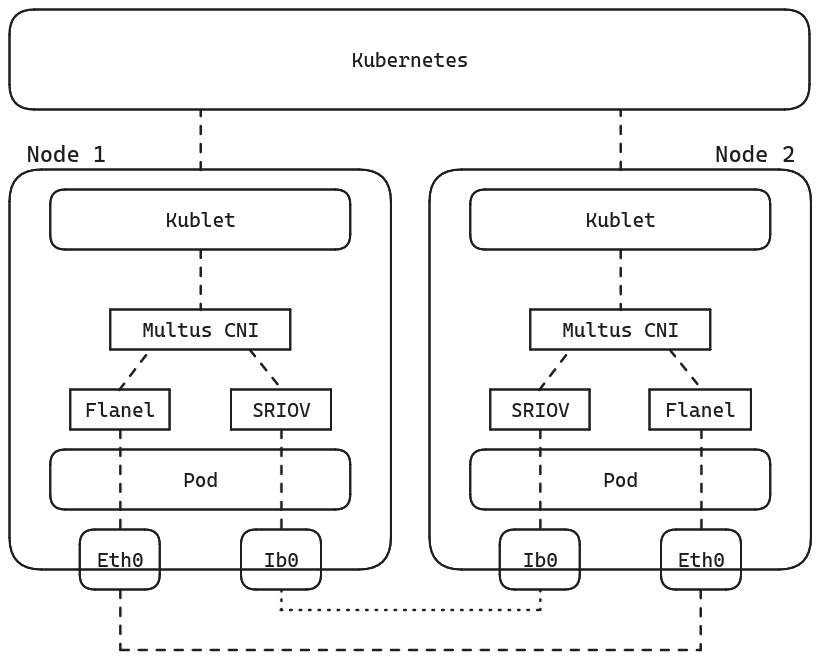
\includegraphics{./graphics/Multus.png}
    }
    \caption{Multus \ac{CNI} with SRIOV and Flannel\protect\footnotemark}
    \label{fig:multus_cni}
\end{figure}
\footnotetext{Based on: \cite{redhatMakingHighPerformance}}



In diagram \ref{fig:multus_cni}, above one can see the end goal of this whole iteration, as this
diagram shows how \textit{Multus} slots itself between the \textit{kublet} and the default \ac{CNI} plugin ,
in hour case \textit{Flannel}, and then plugs in another \ac{CNI} plugin, in this case \textit{SRIOV}
being used to provide the direct access to the \ac{IB} network.

To implement this, the nodes were first \gls{cordoned} and \gls{drained} to ensure that no pods were running on them.
The binaries for \textit{Multus} were compiled and builtd into a container image, which was run as a daemonsets on the cluster.
The container placing accessing the filesystem of the hosts, copying over the binaries, and most importantly
replace the config files of the previous \ac{CNI} plugin and not deleting but deprioritizing them\footcite{multusK8snetworkplumbingwgMultuscni2024a}.
This is done so the \textit{Multus} plugin will be the first to be called by the \textit{kubelet},
when creating a pod; if nothing else is defined the \textit{Multus} plugin will then simply call the default \ac{CNI} plugin,
in this case \textit{Flannel}.

Generally, installing another \ac{CNI} plugin would not be much more complicated as the \textit{Multus} plugin.
Adding the \ac{CNI} binary to all hosts and adding a generic configuration file to the \textit{kubelet} would be enough.
However, as the goal is to connect an \ac{IB} network to the pods, the process is a bit more complicated and will be discussed in the next section.

\pagebreak
\subsection{Evaluation of Results}

Installing the \textit{Multus} plugin was successful, and the plugin was able to run as expected.
Injecting itself automatically between the existing \textit{Flannel} plugin and the \textit{kubelet} worked exactly as expected.


\subsubsection{Utilizing \ac{IB}}

As described in the chapters \Nameref{sec:hpc_infrastructure} and in the design of this prototype \Nameref{sec:suggarch_network},
the Interconnect is a crucial part of a \ac{HPC} system.
Especially so in in \ac{GASNet} systems relying on the low cost \ac{RDMA} based injections to achieve its
global address space (further discussed in \ref{sec:gasnet}).

But Infiniband is by far not as deeply integrated in the Kubernetes ecosystem as the generic \ac{TCP/IP} stack.
As such the process of connecting the \ac{IB} network to the pods is a bit more complicated than just installing a \ac{CNI} plugin.

First the \ac{IB} network needs to be configured and available on the hosts.
The right kernel modules need to be loaded, the right firmware installed and the right \ac{UEFI} settings need to be set.
If all the hardware is set up correctly, and the network has a subnet manager running, the \ac{IB} network should be available on the hosts.

Unlike the \ac{TCP/IP} stack on Kubernetes the \ac{IB} network is not made out emulated
interfaces within the Pod which get routed by the containerized infrastructure until it funnels
out a single interface on the host (as described in \ref{sec:K8sNetworking}).
Instead, the \ac{IB} network is a physical network that
which needs to execute these operations on the hardware level in order to maintain the
extremely low latency and high bandwidth that \ac{IB} networks are known for\footcite{pfisterIntroductionInfiniBandArchitecturea}.

But in order to provide more than one container at a time with isolated access to the \ac{IB} network,
the \ac{IB} network needs to somehow be split up into multiple virtual interfaces for the pods to use.
As this has already been a topic of interest to virtualization technologies, wanting to take
advantage of the low latency and high bandwidth of \ac{IB} networks similar to the pass through
solutions described in the section \Nameref{sec:virtualization}.

\text{SRIOV}:

One such technology is \ac{SRIOV}, which splits a single physical \ac{PCI} into multiple virtual \ac{PCI} interfaces,
which can then be access by different entities on the host, acting as if they were physical interfaces.
These \ac{VF}s can be configured by directly accessing the original \ac{PF} to create the \ac{VF}s as needed.

Both of these still reside in the hosts' kernel space and are not yet available to the pods.
So if a \ac{VF} has been created manually the Pod needs a way to access this \ac{VF} directly.
This is where the \textit{ib-sriov-cni} comes in, as it is a simple \ac{CNI} plugin
that allows a pod to connect to an existing \ac{VF} on the host\footcite{ib-sriov-cni-repoK8snetworkplumbingwgIbsriovcniInfiniBand}.
While this plugin offers access to a \ac{VF} it needs to be
provided with all necessary network information to establish the connection.
This includes everything, from the \ac{PCI} address of the \ac{VF} to access to the \ac{IPAM}
data of the network the \ac{VF} should connect to.
This requires setting up and writing the configuration for each pod on each node manually.
The \textit{ib-sriov-cni} plugin itself simply resides as a binary in the \textit{CNI} directory of the host,
being called upon if \textit{Multus} is instructed to use it for a pod.


\text{SRIOV-Device-Plugin}:

In order to avoid to manually configuring the network data for each pod,
the \textit{SRIOV-Device-Plugin} can be used.
This Kubernetes plugin scans the nodes via a Daemonset for \ac{PCI}
devices which match a given definition and index them.
This creates a resource pool of \ac{SRIOV} devices available to connect to,
which can then be used by the \textit{ib-sriov-cni} plugin to connect to the \ac{VF}s.
Reducing the need to manually declare the data of the \ac{PCI} device manually for each pod.
This needs to be configured with the parameters of the
\ac{PCI} devices to be matched and then run as a Daemonset on the cluster.



\text{Sriov-Network-Operator}:

Now that the pod can automatically discover \ac{VF}s on the host,
the network data configuration for the pods need to be set up,
so that a pod can actually receive the configuration of which network to connect to.
The \textit{sriov-network-operator} is a Kubernetes operator that allows a user to define
a custom resource that describes the desired state of the network configuration of the cluster.
Requesting a specific network devices to provide the necessary \ac{VF}s to the pods.

Once the \textit{sriov-network-operator} pod has been deployed to the head node of the cluster,
it will start a daemon on each node which keeps track of the state of each node and the network
devices ready to be used by the \textit{ib-sriov-cni} plugin. It also sets up endpoints
for the KubernetesAPI to interact with the \textit{sriov-device-plugin}.

Once a user creates an instance of the custom resource called \textit{SriovNetworkNodePolicy},
the \textit{sriov-network-operator} will create a \textit{NetworkAttachmentDefinition} object
which will can be referenced in the pod configuration as an annotation.
While in the background the \textit{sriov-device-plugin} on the nodes register the difference between
desired and actual state of the network devices, and signals the KubernetesAPI to update the state of the
Node. The Api then calls on the \textit{sriov-network-operator} to update the configuration.


Once the \ac{VF}s are available a pod can be created with only the name of
the network to connect to, the once a pod with the right keyword is requested, the
resource injector matches the network name with the existing \textit{NetworkAttachmentDefinition}
and injects the necessary information into the pod configuration.
Using this configuration the \textit{Multus} plugin then knows to call the \textit{ib-sriov-cni} plugin
providing the injected network information to the pod.


\begin{figure}[!ht]
    \vspace{0.8cm}
    \centering
    \scalebox{0.35}{
        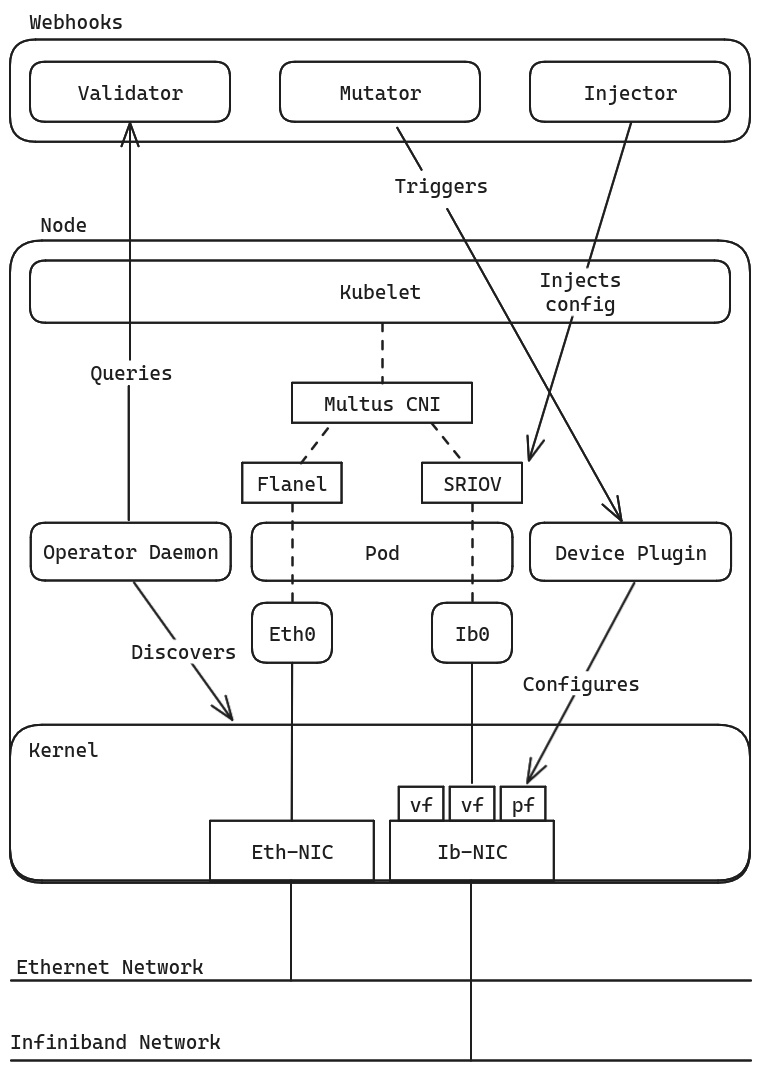
\includegraphics{./graphics/SRIOV Infrasturcture.png}
    }
    \caption{Simpliefied architecture of a SRIOV enabled Kubernetes Node}
    \label{fig:Sriov_infrastructure}
\end{figure}

In diagram \ref{fig:Sriov_infrastructure} above, a simplified version of the interactions within a single node of the cluster is shown.
Not pictured are the daemons running on the head node or, calls of the Kubernetes API, or the mutating
config maps which are being mutated by the system to declare the current and desired states of the network devices.

\textbf{Implementation process}

During the implementation of this iteration many problems arose in orchestrating these many interdependent components.
As the use case for \ac{IB} enabled \ac{HPC} on Kubernetes has not been widely explored, many of the components
are originally intended for other use cases, unmaintained or proprietary. A large part of the existing documentation
was addressed at fellow developers, describing the necessary steps built the components, but do not
provide information about how to deploy or configure them, as this is assumed to be known by the developer of the
component in the first place. This made the process of setting up the \ac{IB} network on the cluster a very
time-consuming and painstaking process, involving a lot of reverse engineering and trial and error, sometimes
discovering known caveats documented only as a side note in the source code of the component.
The most helpful resource was \textit{Redhat}s documentation\footcite{redhat-openshiftSingleRootVirtualization} for their \textit{OpenShift} platform,
their custom Kubernetes based platform. While useful and detailed, their documentation is only targeted
at their platform and the translation to vanilla Kubernetes is not always straightforward.

Amongst the issues encountered was a communication problem, between the Kubernetes API and the
sriov-operator-webhook-config \textit{mutatingwebhookconfigurations} and its \textit{validatingwebhookconfigurations}.
While the webhook was configured according to the documentation, the underlying pod was able to receive
and log requests and the provided certificates were valid, signed and concurrent between the webhook and the container
the API was getting a "500 Internal Server Error - Bad Gateway" when trying to reach the webhook. This behavior
could not be reproduced in any other way during debugging.
While the issue was worked around at first by overwriting the webhook, it was later coincidentally discovered that
The system requires the filename of the certificate file to be identical to the secret containing the file.
While a banal issue, it was only documented in form as a comment in the code of the webhook itself\footcite{sriov-network-operator-repoSriovnetworkoperatorBindataMaster}.

The most Significant hurdle was the in transparent configuration of the \ac{IB} device and the components directly
interacting with it. As there is little community effort behind these projects and numerous proprietary
components involved, the configuration of the \ac{IB} device was the part of the prototyping process which
cased the project to hit the deadline for the prototyping process, requiring the project to be continued
after release of this paper.

\textbf{Current State}

While the above described infrastructure has been set up and brought to a working state,
completely enabling the configuration of the cluster by declaring the required configuration of the
nodes and declaring a network. Even the mounting of the \ac{IB} network to the pods has been achieved.
And while the \ac{VF} functions are accessible and intractable by the pods, the pods are not able to
able to send or receive data over the \ac{IB} network.
This is due to the interface requiring the \ac{RDMA} module requiring to be set to the \textit{"exclusive mode"}.
While setting the device to exclusive mode is a simple command, this in turn disables the \ac{VF}s completely.
While this is most likely a trivial configuration issue, the deadline of the prototyping process has been reached
and this paper is to be handed in. The project will be continued after the release of this paper.
The current state of the project can be found in the corresponding repository and will be updated as
the project progresses\footcite{joneckerthBachelorsThesisProjectMain}.

\subsection{Conclusion}

While the setup of the infrastructure as a whole was successful within on the Kubernetes Level,
the many small issues resulted in the project running out of time, without being able to
fully set up the hardware and kernel level configuration of the \ac{IB} network.
The original goal of this iteration was to enable the \ac{IB} network to be used by the pods,
in order to enable a high speed low latency network for the \ac{HPC} applications.
This goal has not been achieved, as the pods are not able to send or receive data over the \ac{IB} network,
without the correct configuration of the \ac{IB} device.
While this iteration was not finished, this is not due to any insurmountable technical reason,
but rather due to the time constraints and the complexity of the set up the infrastructure.

Comparing this state to the our original design,
the set up has come very close to the original intention,
as it was already suspected that a multi network infrastructure might be necessary.
While it was originally planned to use the Singularity \ac{CNI} in order to provide the
native \ac{IB} support, its abandonment by the community required the
use of a manual integration of the necessary components into the cluster.
But even in the case a dual \ac{CNI} setup would have been needed to provide the
necessary network abstraction for the standard Kubernetes functionality
to function with the \textit{Singularity} containers.

While there will be no additional iterations in this paper,
the project will be continued further, both to achieve the
original design goal, as well as to follow up on the opportunities
described in the section \Nameref{sec:future_work}.

Therefore the next undocumented iteration will first focus on
configuring the \ac{IB} network to be accessible by the pods and
compare the performance of the \ac{IB} network to the standard
established during the second iteration.

\pagebreak

% Conclusion
\section{Conclusion of the Prototyping Process}

As the goal of this chapter was not just to create a usable artifact for its own right
and explore the process of building a kubernetes-based \ac{HPC} tool,
but also to stand as the validation step of the system designed in the \Nameref{suggested_architecture}.

While each iteration of the prototyping process is split into goal, implementation, and evaluation
sections, this section serves to do this for the process as a whole and conclude not just the prototyping process,
but the conceptual design of the system as a whole,
by reevaluating the original design with the insights gained from the prototyping process.


\subsection{Summary of the Prototyping Process}

Before the three iterations of the prototyping process are set up, executed and evaluated,
the existing infrastructure, previous work, and the environment of the prototyping process are described.
This is done to set the stage for the prototyping process, as well as to
highlight the first differences between the suggested architecture and the prototype to be.
This is important as the architecture is designed from a deductive standpoint,
being a system that is supposed to be generic and not influenced by previous decisions.
Confronting this design with the first practical steps is the first step in the validation process.
From this the changes extensions and removals of the previous system are derived.

The fist iteration (\ref{sec:iteration_no1}) of the prototyping process is to create the most basic version of the system,
possible, to test the feasibility of the system and the environment.
This is done by verifying the operative state of the system and the environment,
fixing issues with the existing infrastructure.
For the basic functionality of the system, a custom container image is created,
containing the necessary tools and libraries to host a Notebook server.
Using a modified \textit{Ipython} kernel, the Arkouda and Chapel libraries are
integrated into the container which automatically connect to the compute nodes when
activated. To make the system able to be used on the cluster a deployment and a
service are created, to make the system accessible from the outside.
The system is then tested by running a simple example, to verify the functionality of the system,
some issues are then identified and workarounds are implemented to create the first working version of the system.

As the first iteration  has successfully implemented a \ac{MVP} of the system,
second iteration (\ref{sec:iteration_no2}) aims to improve the system as
the previous version did not regard speed and stability as a priority.
During this iteration the previously created notebook container is rebuilt in
order to optimize the performance of the system.
The infrastructure from the previous iteration is then given the same treatment,
completely rebuilding the entire container images from scratch in order to
reduce their size and to remove version mismatches in the underlying libraries.
To measure these improvements the deployment times of the system are benchmarked.
Additionally it was attempted to replace the \ac{CRI} with a faster \ac{HPC} oriented
one, which was not successful due to kubernetes dropping support for the \ac{API}
specification which the \ac{CRI} was based on.
Even though the \ac{CRI} could not be replaced, the system was still benchmarked
to measure the compute node's performance and to identify bottlenecks in the system
For this purpose a simple benchmarking framework was converted to a deployment
capable of running in a kubernetes cluster and to interact with the compute nodes
to measure the performance of the system.

The goal of the third iteration (\ref{sec:iteration_no3}) was to move the system from
a simple proof of concept to a system which could not just technically solve \ac{HPC} problems,
but one that is not constrained by consumer level hardware, so its performance can be
compared to an equivalent section of a real system.
While the previous section had the goal of implementing \textit{Singularity} to
make use of its near native performance, it was also hoped to make use of its
native support for \ac{IB} to make the third iteration much easier to implement.
But as \textit{Singularity} was not supported the \ac{IB} was implemented manually
using a multitude of different tools and configurations in order to properly provision
and integrate the device into the Multi \ac{CNI} setup, installed to enable the usage.
During the integration of this step the prototyping was cut short due to the time
constraints of the thesis, leaving the \ac{IB} integration for future work.
But as the flannel \ac{CNI} is still completely in place the system is still
fully functional and can be used to run \ac{HPC} workloads using the \ac{TCP/IP} protocol.


\subsection{Evaluating against the Deductively Designed System}

As the prototyping process is now concluded and summarized,
it is time to complete the validation of the deductively designed system
and to evaluate the prototyping process against the original design;
contrasting the theory with practical implementations, which changes
where made out of incorrect assumptions and which where made out of necessity,
and which are improvements of the general design.

The following section will go through the different aspects defined in the
\Nameref{suggested_architecture} and evaluate them.


\textbf{\hyperref[asp:client]{Client}}:

In the design it was assumed that the client of the user would
be a local interface of Jupyter notebook, which would be connected to the
server via a web interface.
This assumption has been implemented int the prototype and even used during the
data analysis of the prototyping process.
Beyond having a local interface, such as a local Jupyter notebook or the \textit{VSCode} extension,
the system can just as easily be accessed from a web browser,
making it highly accessible and and flexible in its use.
The original design has been validated by the prototyping process.

\textbf{\hyperref[asp:language]{Language}}:

In the original design it was decided to make this project Arkouda first,
as it is a modern and easy to use way of interacting with the \ac{HPC} system.

While Arkouda itself is very user friendly and easy to use, the installation,
needing to have a precompiled Chapel version, and then manually compiling
and importing the Arkouda library, is less so.

While this made the creation of custom containers more complicated,
form the perspective of the user, the system is now as easy to use as
native python on any jupyter notebook server, making the system very user friendly.

From the perspective of compute performance, the system was as efficient as
the underlying infrastructure permitted, being bottlenecked by the
networking (see \Nameref{sec:performance_testing}).

There is no reason to discount the original decision to use Arkouda as the
primary language of the system.


\textbf{\hyperref[asp:cluster]{Cluster}}:

The original design assumed that the system should be run on a Kubernetes cluster,
while this is an integral part of the ability to scale the system,
the prototyping has shown that Kubernetes is not build for connecting
easily to hardware devices which are standard in \ac{HPC} environments.

Integrating these devices is a major challenge and when deciding on
building a cloud native \ac{HPC} system, it should be strongly considered
wether a Kubernetes cluster is the right choice for the system,
or whether the other opportunity discussed in this section should be used.
This being the bare the orchestration of bare metal systems.

So while the design inherently relies on the use of a Kubernetes cluster,
and therefore it needs to be included in the system, this is a
decision that should only be made if the high flexibility
and scalability of containers is needed.

\textbf{\hyperref[asp:jupyter_server]{Jupyter Server}}:

The original design discuses the decision between using a simple Jupyter server
or a whole JupyterHub setup, the prototyping process has shown that
the setup of a single Jupyter server is sufficient for the system,
and quite uncomplicated to set up.

Orchestrating a single or a few JupyterHub in oder to manage multiple users
would increase the complexity of the system, while the use of a single Jupyter server
per user is a much simpler solution, which is sufficient for the current goals of the system.

This decision is validated by the prototyping process.

\clearpage

\textbf{\hyperref[asp:compute_services]{Compute Services}}:

As Arkouda was already selected the choice of compute service was obvious,
as the Arkouda Client is build to interface with a Chapel backend, through the
Arkouda server witch wraps the Chapel library.

While the same limitations exist for the Arkouda server as for the
Arkouda client, needing to compile Chapel and Arkouda manually, making
an iterative development process more complicated, the experience during
runtime is user-friendly and and relatively quick, considering the
networking limitations of the system.

The original design has been implemented as described and is a valid choice for the system.
But further optimization of the system could be considered to ease and speed up the
development process, as many steps of the initial setup are still required to be done manually.
A more automated and consolidated setup would be beneficial for both the scalability and the
maintainability of the system.

Over all, the original design is validated by the prototyping process, and further potential
has been identified.

\textbf{\hyperref[asp:resource_provisioning]{Resource Provisioning / Scaling}}:

Original goal of the system in the design was to dynamically scale the system,
either on a job by job basis or by scaling the based on sessions.

While the system can be rescaled via a single variable in between sessions,
this feature has not yet been implemented deeply enough in the system.
It's implementation during later iterations was a significant factor in the decisions
made during the earlier stages of the prototyping process, such as setting
up the self configuring implementation of \ac{IB}, the optimization of the container images,
and the one notebook per user setup.

While this feature has been deemed important for the system the decision to
make all parts scalable from the beginning should be reconsidered.
Creating a system that is at first not scalable, but completely functioning
with all the relevant features and then optimizing the necessary parts for
scalability. Would have resulted in more insights early on in the prototyping process,
but would have created more work over all.
Under the light of the time constraints of the thesis, the decision to
prioritize the scalability in each step component of the system has lead to
not reaching the goal of a fully scalable system, in the time frame of the thesis.

Therefore, while the original design is valid, it should have been differently prioritized.


\textbf{\hyperref[asp:operating_system]{Operating System}}:

The original design assumed that the system would be run on a Linux based system,
which is a necessary and valid assumption, for both Kubernetes and \ac{HPC} systems.
This part is validated by the prototyping process.

A second consideration was wether to use a generic Linux distribution or a specialized one,
while the choice of a generic distribution has been sufficient for the prototyping process,
choosing a licensed distribution specialized in this sector of Kubernetes would have
enabled the access to more specialized support and documentation, which would have
speed up the prototyping process significantly.
On the other hand the use of a non generic distribution entails the reliance on
licensed software, which would have made the system less accessible to the general public.
And setting up the entire cluster from a blank system offers a much deeper understanding
of the system as a whole, which is invaluable for the development of the system.

Therefore both decisions are equal valid and the choice between them should be made
depending on the goals of the developer, for a more flexible and public system a generic
distribution would be the better choice, while for a licensed and specialized system
will provide benefits for production systems.

This decision is validated by the prototyping process.


\textbf{\hyperref[asp:container_runtime]{Container Runtime}}:

During the design phase three different container runtimes where picked out as
possible candidates on which the system could be run.

On the baseline either \ac{CRI-O} or \textit{Containerd} where considered with
\ac{CRI-O} being the preferred choice due to its closer accordance with the
\ac{OCI} specification.
As an additional option \textit{Singularity} was considered as a runtime
for the compute pods to use its performance benefits.

As the previous system was already running on \textit{Containerd} and the
benefits of \ac{CRI-O} where not significant enough to warrant the change,
the decision was made to keep the system on \textit{Containerd}.
Not invalidating the original proposal but diverting from it out
of practicality.

The decision to include \textit{Singularity} as a secondary runtime,
on the other hand was inherently misinformed, as is described in the
section \Nameref{sec:container_runtime}.
Going down this path is not recommended, as either an unsupported version
of Kubernetes would have to be used, or the \textit{Singularity} \ac{CRI}
would need to be patched.

In conclusion the original design is validated in regards to the base container runtime,
but the decision to include \textit{Singularity} has been completely invalidated.

\textbf{\hyperref[sec:container_image]{Container Image}}:

As touched upon in the compute services section, the container images used where
based on the ones provided in the contributions repository of the Arkouda project.

While they have been an excellent starting point, the prototyping process has shown that
the images where able to be be significantly reduced in size and optimized for the system,
which has improved the performance of the system.

One significant change needed to be made in the future is to create a set of \ac{IB}
capable images, as this needs to be set up during compilation time and can not be
changed during runtime.

The original design has been validated by the prototyping process and has been improved upon,
and still has potential for further improvements.

\textbf{\hyperref[asp:network_abstraction]{Network Abstraction}}:

During the original design the tradeoff common network abstraction layers make
between performance and flexibility was highlighted and it was concluded that a
multi \ac{CNI} setup would be an essential part of the system.

Creating two separate network, one for the orchestrating communication, and one
to provide the high-speed \ac{RDMA} capable communication the \ac{HPC} components
require.

It was already recognized that for this setup to work a meta \ac{CNI} such
as \textit{Multus} would be necessary to enable the use of both networks.

While the need for this system has been thoroughly shown during the prototyping process,
and the implementation of a dual \ac{CNI} setup was has been proven as the only valid solution;
Other solutions such as keeping the original \textit{Flannel} \ac{CNI} and
facilitating the \ac{RDMA} communication on the container runtime level where considered but
have been proven to be infeasible.

While the original proposal on the network abstraction level has been implemented, via
the use of a dual \ac{CNI} setup, the ramifications for the configurations of the underlying
hardware where severely underestimated, which will be discussed in more detail in the paragraph
\hyperref[par:network_interconnect]{"Network Interconnect"} of this section.

Overall using a dual \ac{CNI} setup is a valid solution if the requirements of the system
demand a high-speed \ac{RDMA} network, a containerized environment and a flexible communication
infrastructure.

If this is not the case, a bare metal ethernet network, running the workload directly on the system
or a fixed network configuration should be considered instead.

\textbf{\hyperref[asp:compute_node_hardware]{Compute Node Hardware}}:

In the effort to create a generic design, only generic recommendations where made
during the design phase, especially as the system, using containerization is
largely hardware agnostic.

As the network revealed itself to be the main bottleneck of the system, the
compute and memory specification of the system did not impact the performance
in a significant negative way.
This is demonstrated by the fact that during the performance testing \ac{PGAS}
memory occupation did not exceed 30\% of the available space when
the 10Gbit network was at its maximum capacity.

But nevertheless, the memory speed and capacity, as well as the \ac{CPU} performance and \ac{NUMA}
topology of the two socket nodes would most likely be of significant importance
after the implement of a dedicated \ac{IB} network.

The other aspect discussed, being the capability of respecting non homogeneous
systems was important during the building and testing of the network abstraction.
Using a hardware scanning daemonsets, to identify available hardware made it
easy to segment the deployments to either the \ac{IB} capable or in capable nodes,
by simply stating the need in the configuration.

While not proven during the prototyping process, the assumption that a
more compute capable system would be able to handle more workloads still stands.
On the other hand it was shown that the use of heterogeneous systems is possible,
as special need hardware can be reserved for special workloads if needed,
but is fully capable of running pods with on all nodes, independent of
the underlying hardware.

Validating the latter and not invalidating the former, part of the original design.

\textbf{\hyperref[sec:suggarch_network]{Network Interconnect}}:
\label{par:network_interconnect}

As has previously been referenced, one of the major bottlenecks of the prototype was
the network. This was already correctly anticipated during the design phase and
the decision to utilize an \ac{IB} network interconnect was made.

During the design phase it was assumed that the installation of the \ac{IB} network,
would be of equal complexity as any other \ac{CNI} addon; not trivial but manageable.

But this notion was shown to be incorrect, as the setup of the \ac{IB} network
and the necessary multi layered infrastructure to configure it through Kubernetes
was a major challenge took up a significant amount of time during the prototyping process.

While the Kubernetes side of the setup has now been brought to a working state,
the configuration of the necessary kernel modules has been cut short due to
time constraints of the thesis.

While the reason for the \ac{IB} interconnect is valid; bringing the performance from
acceptable for medium sized workloads, to good performance for large scale \ac{HPC} workloads.
The complexity of this setup was severely misjudged and resulted in a major disruption
of the time schedule of the prototyping process, resulting in features not being implemented
and the original design not being able to be fully validated.

One of these features is the dynamic scaling of the system, which would have lead to
the investigation of the need for topological awareness, which has also been discussed
in this section of the design.

While the need for a high-speed network interconnect has manifested as expected,
the applied solution was not feasible in the time frame of the thesis.
Instead it is recommended to either circumvent the need for a \ac{IB} integration,
or to allot this step the necessary resources to be implemented correctly.
This could be done by making use of enterprise support, hiring a specialist
or allotting more time to the prototyping process.
Regarding the network topology, no evaluation can be made, as neither
a state in which the need could be evaluated nor a test setup has been reached.


\textbf{Conclusion}

Circling back to the original goal of the Conceptual Deductive Design,
as defined in \Nameref{sec:goals}:

\textit{\say{The designed system should provide the user with a easy to use interface,
        capable of interactively exploring HPC scale data.
        The system should be able to run on cloud infrastructure, be able to
        to allocate the necessary resources, as well as scheduling and executing
        the computation within a reasonable time frame.}}

This prototyping process has shown that this goal is technically feasible,
and has largely been achieved. While two of the design goals where based on
incorrect assumptions, most have either been validated or even expanded
upon during the prototyping process.

These divergences between a theoretical design and the realities of an
actual implementation, have now been either been corrected, put in
a more appropriate context or have been proven to be based on incorrect
assumptions.

Overall the design as well as the prototyping process has been a success,
as the central functionality of an interactive system was successfully implemented,
but most importantly valuable insights have been gained about the prototyping process
as well as the cavitates of a deductively designed system.
Also a useful system has been created which was used to run the data analysis
While there is still work to be done and much long term potential for
the project as a whole, what has been done builds a solid foundation
and many paths forward.



\pagebreak